\documentclass{article}
\usepackage{amsmath}
\usepackage{amsfonts}
\usepackage{amssymb}
\usepackage{multicol}
\usepackage{graphicx}
\usepackage{lipsum}
\usepackage{float}
\title{PowerDecrease}
\author{Jakub Matl}
\date{\today}
\begin{document}
\maketitle
\begin{multicols}{2}
\begin{figure}[H]
\centering
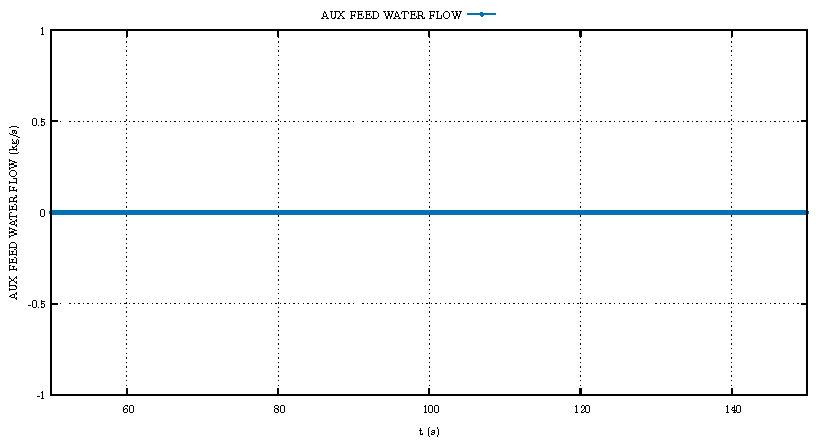
\includegraphics[width=\linewidth]{./graphs/AUX FEED WATER FLOW_comp.pdf}
\end{figure}
\begin{figure}[H]
\centering
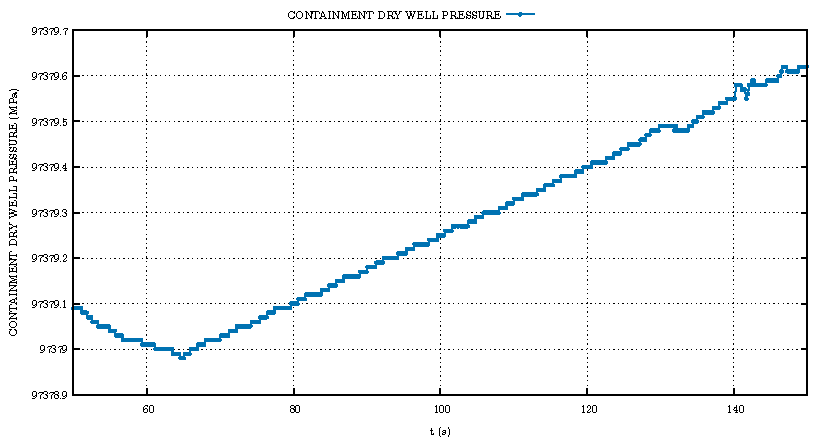
\includegraphics[width=\linewidth]{./graphs/CONTAINMENT DRY WELL PRESSURE_comp.pdf}
\end{figure}
\begin{figure}[H]
\centering
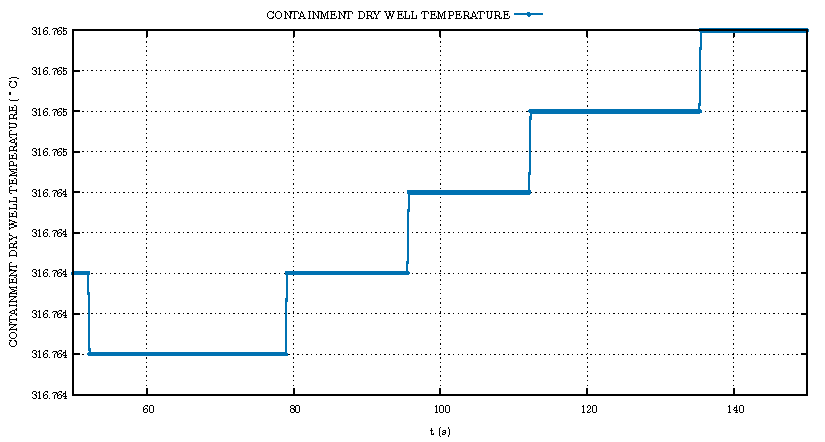
\includegraphics[width=\linewidth]{./graphs/CONTAINMENT DRY WELL TEMPERATURE_comp.pdf}
\end{figure}
\begin{figure}[H]
\centering
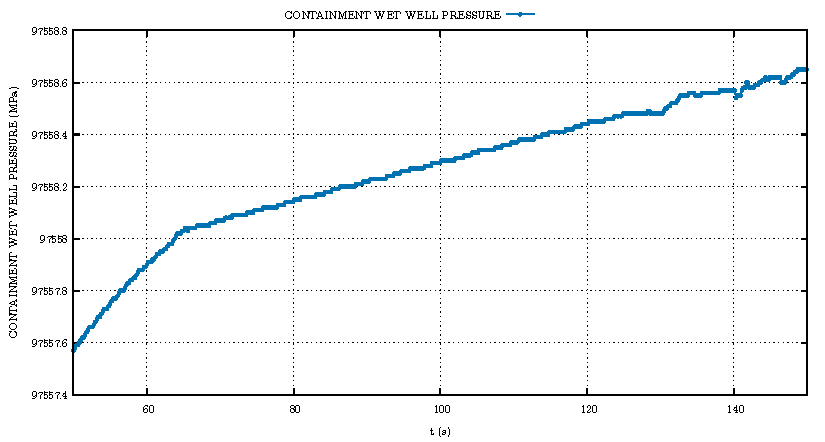
\includegraphics[width=\linewidth]{./graphs/CONTAINMENT WET WELL PRESSURE_comp.pdf}
\end{figure}
\begin{figure}[H]
\centering
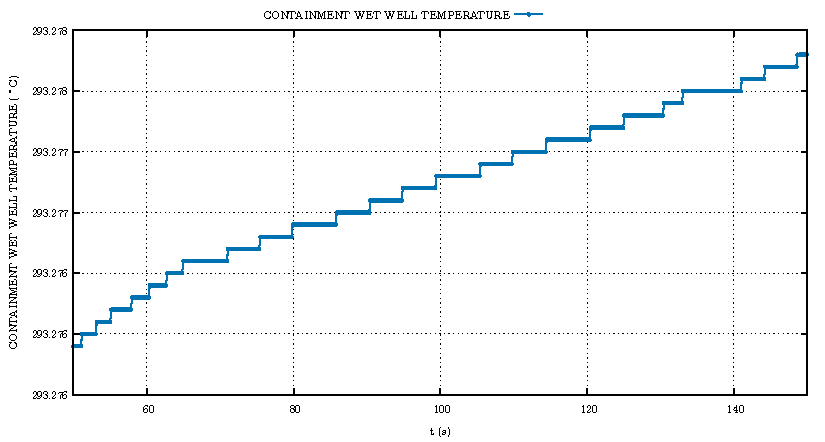
\includegraphics[width=\linewidth]{./graphs/CONTAINMENT WET WELL TEMPERATURE_comp.pdf}
\end{figure}
\begin{figure}[H]
\centering
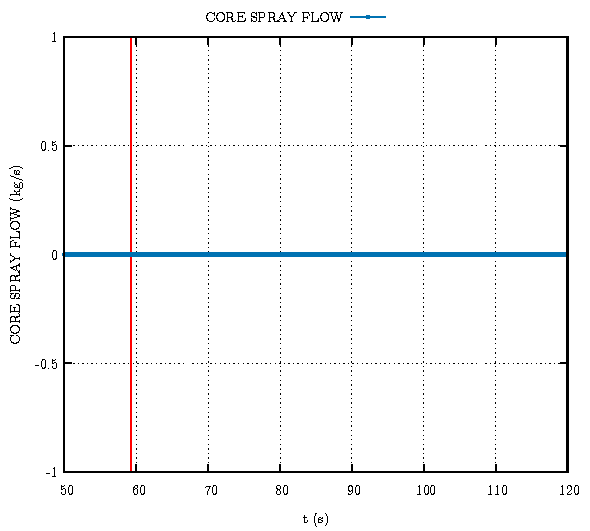
\includegraphics[width=\linewidth]{./graphs/CORE SPRAY FLOW_comp.pdf}
\end{figure}
\begin{figure}[H]
\centering
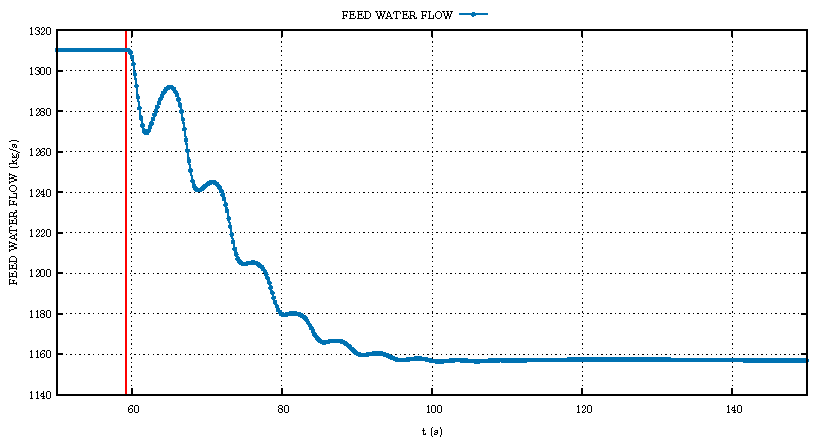
\includegraphics[width=\linewidth]{./graphs/FEED WATER FLOW_comp.pdf}
\end{figure}
\begin{figure}[H]
\centering
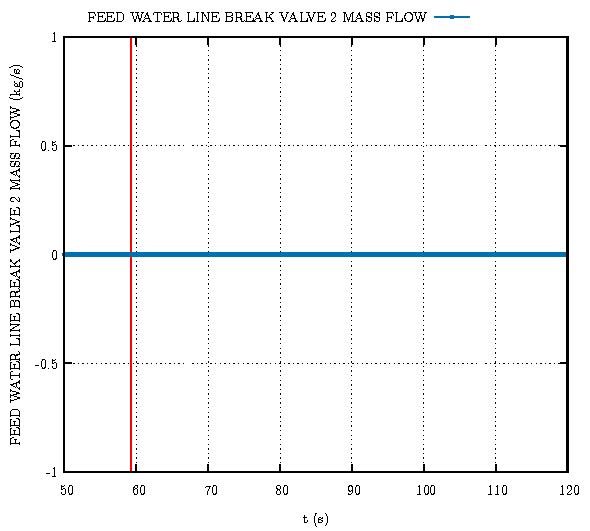
\includegraphics[width=\linewidth]{./graphs/FEED WATER LINE BREAK VALVE 2 MASS FLOW_comp.pdf}
\end{figure}
\begin{figure}[H]
\centering
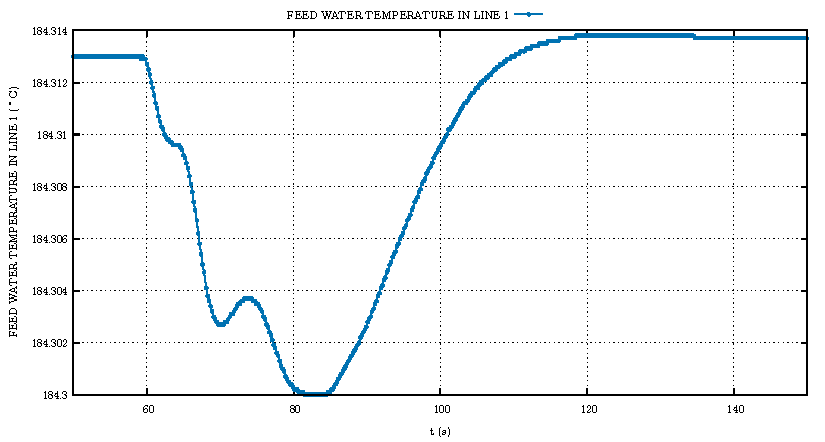
\includegraphics[width=\linewidth]{./graphs/FEED WATER TEMPERATURE IN LINE 1_comp.pdf}
\end{figure}
\begin{figure}[H]
\centering
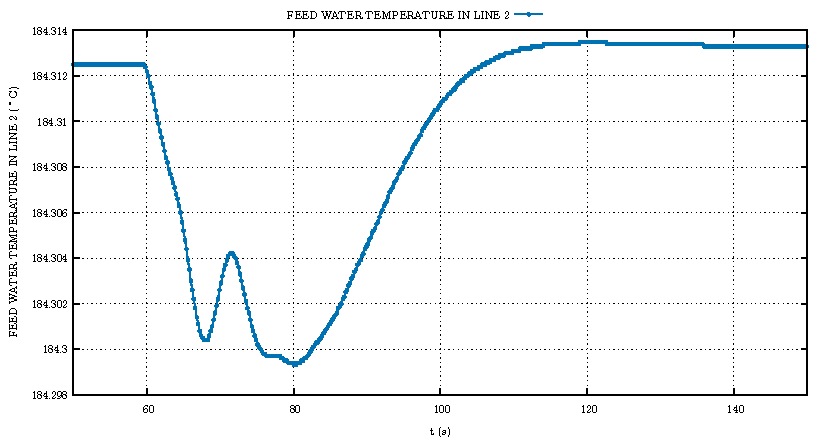
\includegraphics[width=\linewidth]{./graphs/FEED WATER TEMPERATURE IN LINE 2_comp.pdf}
\end{figure}
\begin{figure}[H]
\centering
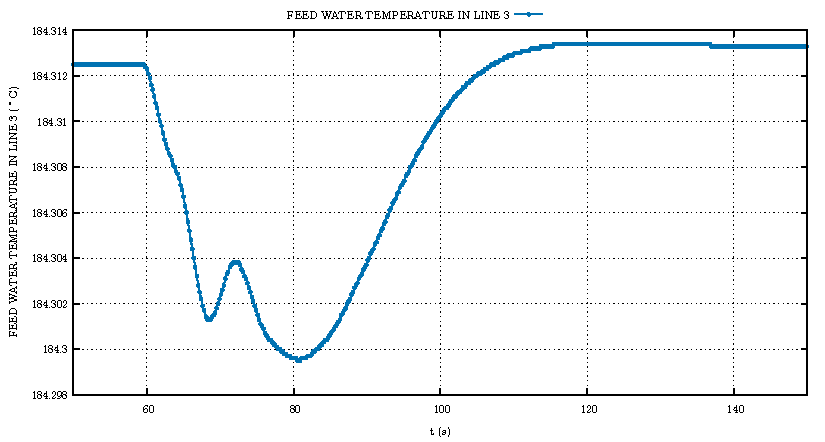
\includegraphics[width=\linewidth]{./graphs/FEED WATER TEMPERATURE IN LINE 3_comp.pdf}
\end{figure}
\begin{figure}[H]
\centering
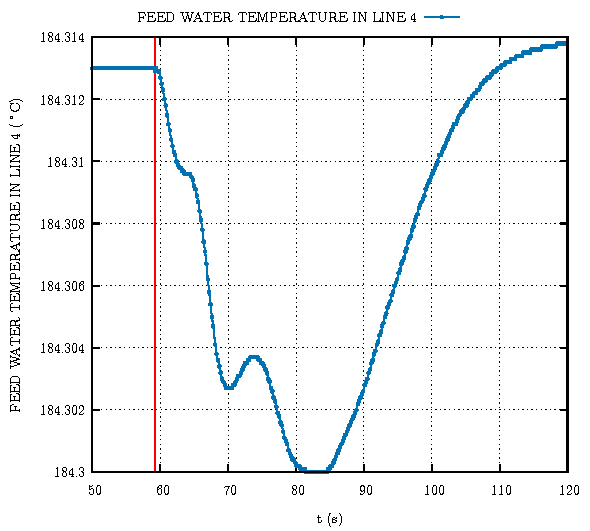
\includegraphics[width=\linewidth]{./graphs/FEED WATER TEMPERATURE IN LINE 4_comp.pdf}
\end{figure}
\begin{figure}[H]
\centering
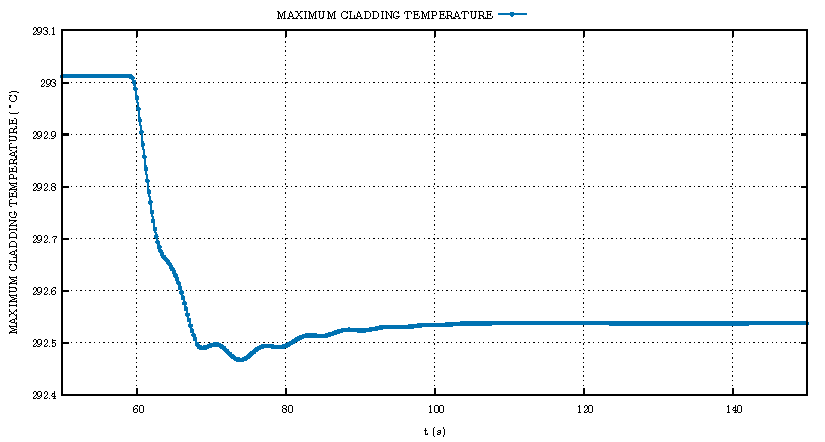
\includegraphics[width=\linewidth]{./graphs/MAXIMUM CLADDING TEMPERATURE_comp.pdf}
\end{figure}
\begin{figure}[H]
\centering
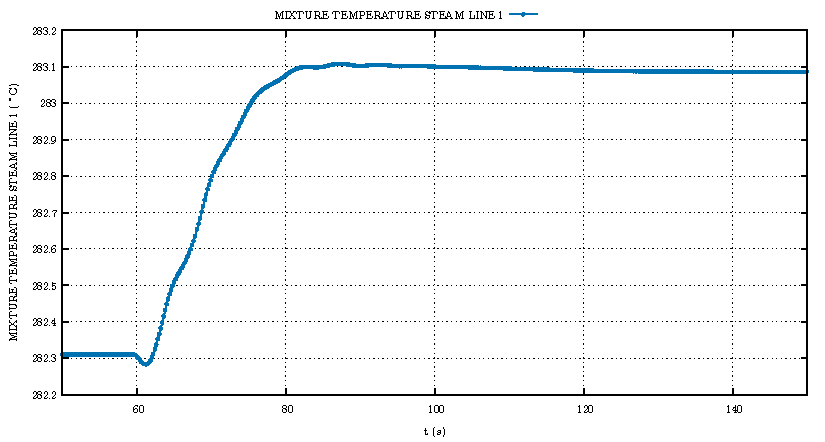
\includegraphics[width=\linewidth]{./graphs/MIXTURE TEMPERATURE STEAM LINE 1_comp.pdf}
\end{figure}
\begin{figure}[H]
\centering
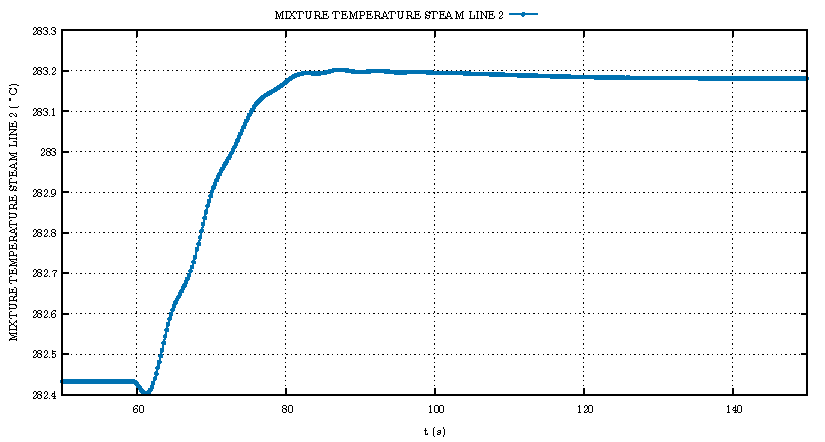
\includegraphics[width=\linewidth]{./graphs/MIXTURE TEMPERATURE STEAM LINE 2_comp.pdf}
\end{figure}
\begin{figure}[H]
\centering
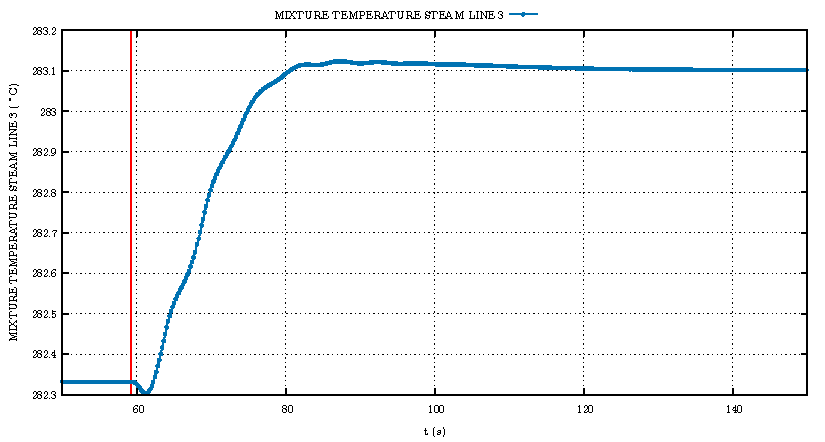
\includegraphics[width=\linewidth]{./graphs/MIXTURE TEMPERATURE STEAM LINE 3_comp.pdf}
\end{figure}
\begin{figure}[H]
\centering
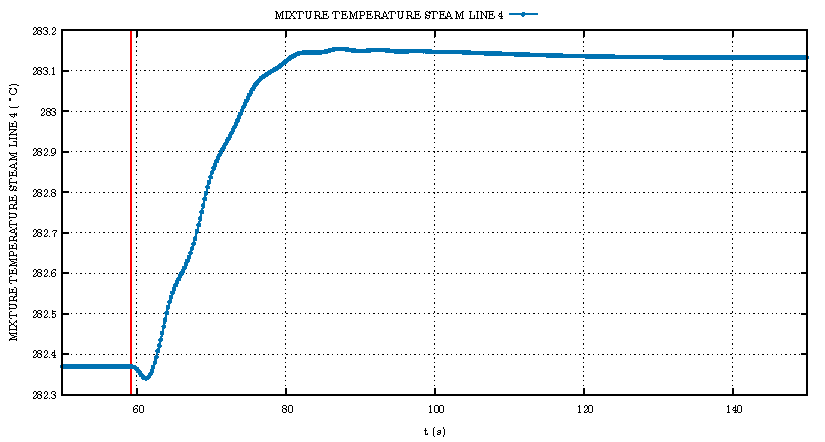
\includegraphics[width=\linewidth]{./graphs/MIXTURE TEMPERATURE STEAM LINE 4_comp.pdf}
\end{figure}
\begin{figure}[H]
\centering
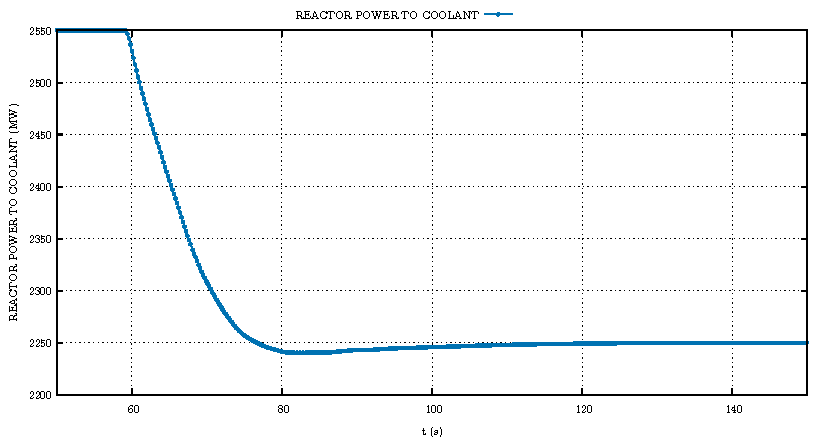
\includegraphics[width=\linewidth]{./graphs/REACTOR POWER TO COOLANT_comp.pdf}
\end{figure}
\begin{figure}[H]
\centering
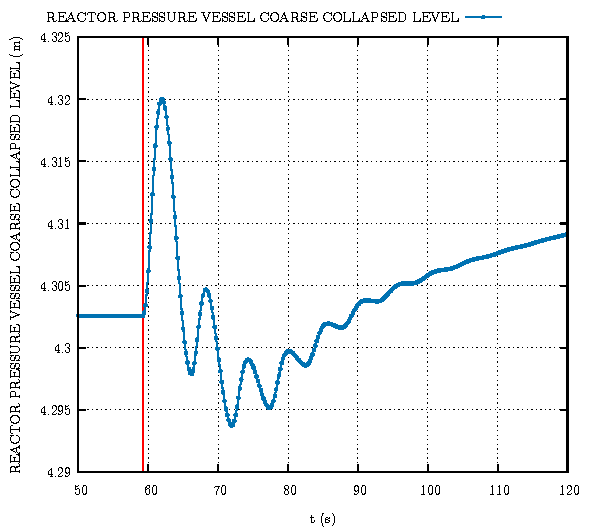
\includegraphics[width=\linewidth]{./graphs/REACTOR PRESSURE VESSEL COARSE COLLAPSED LEVEL_comp.pdf}
\end{figure}
\begin{figure}[H]
\centering
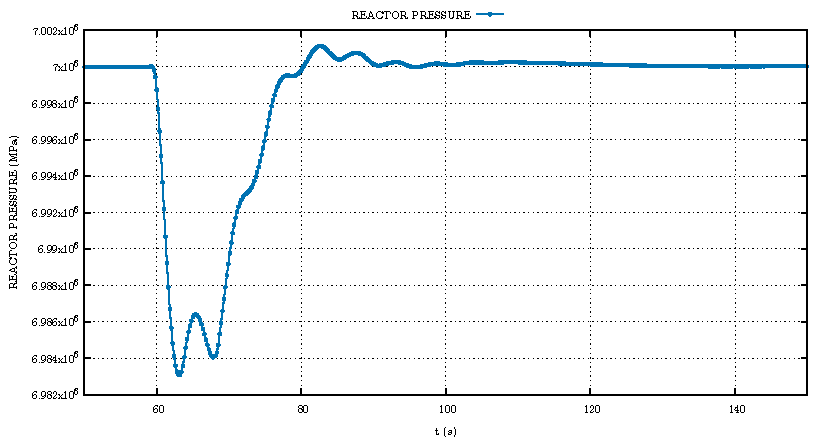
\includegraphics[width=\linewidth]{./graphs/REACTOR PRESSURE_comp.pdf}
\end{figure}
\begin{figure}[H]
\centering
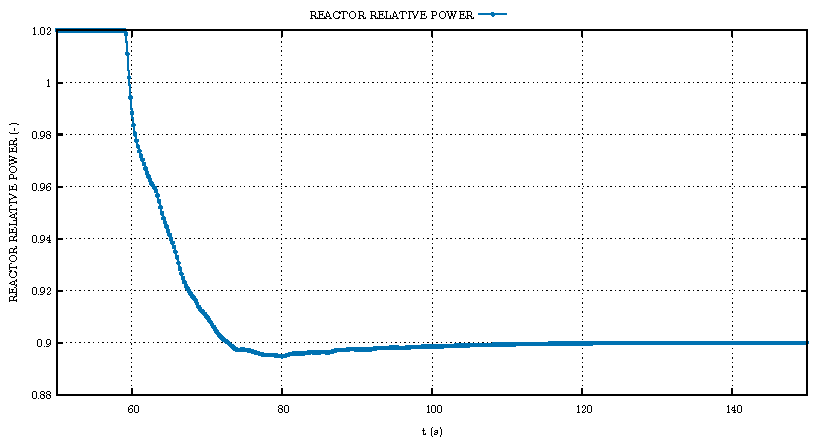
\includegraphics[width=\linewidth]{./graphs/REACTOR RELATIVE POWER_comp.pdf}
\end{figure}
\begin{figure}[H]
\centering
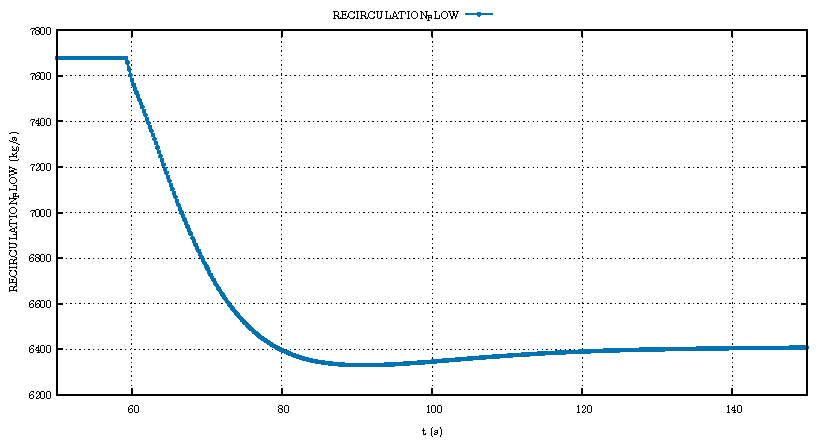
\includegraphics[width=\linewidth]{./graphs/RECIRCULATION_FLOW_comp.pdf}
\end{figure}
\begin{figure}[H]
\centering
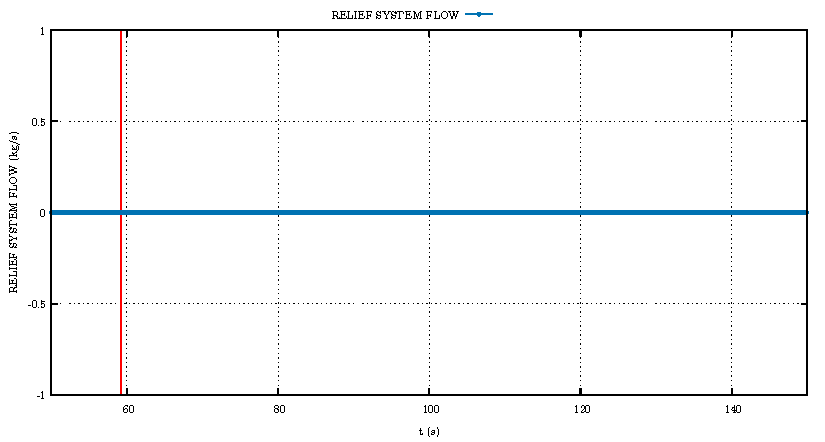
\includegraphics[width=\linewidth]{./graphs/RELIEF SYSTEM FLOW_comp.pdf}
\end{figure}
\begin{figure}[H]
\centering
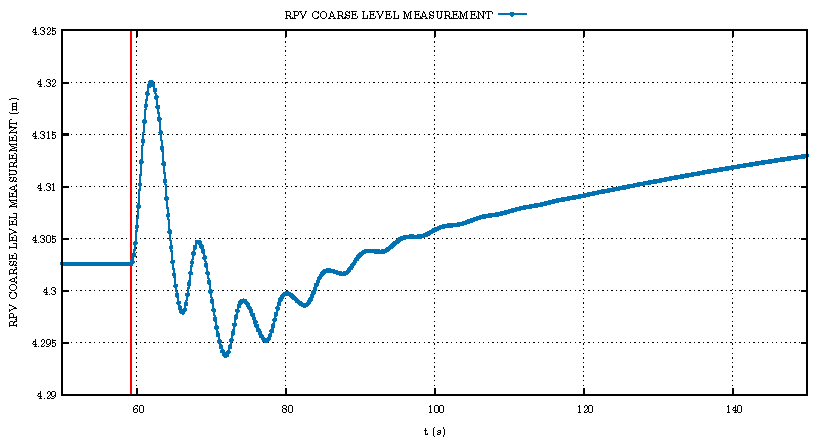
\includegraphics[width=\linewidth]{./graphs/RPV COARSE LEVEL MEASUREMENT_comp.pdf}
\end{figure}
\begin{figure}[H]
\centering
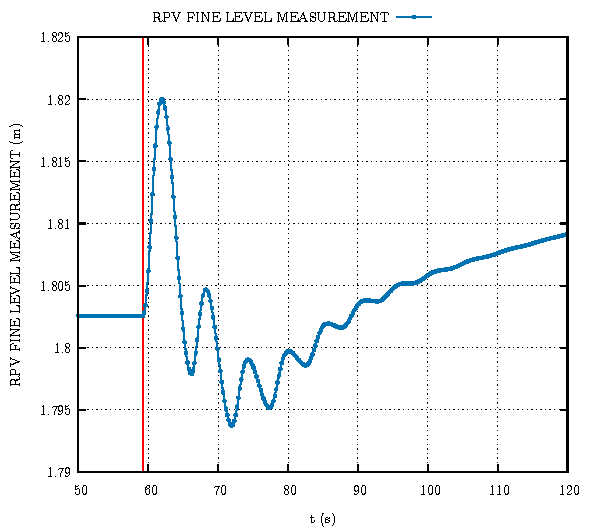
\includegraphics[width=\linewidth]{./graphs/RPV FINE LEVEL MEASUREMENT_comp.pdf}
\end{figure}
\begin{figure}[H]
\centering
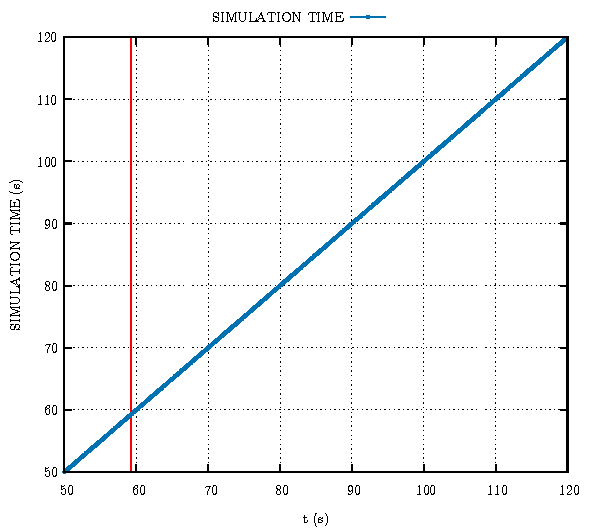
\includegraphics[width=\linewidth]{./graphs/SIMULATION TIME_comp.pdf}
\end{figure}
\begin{figure}[H]
\centering
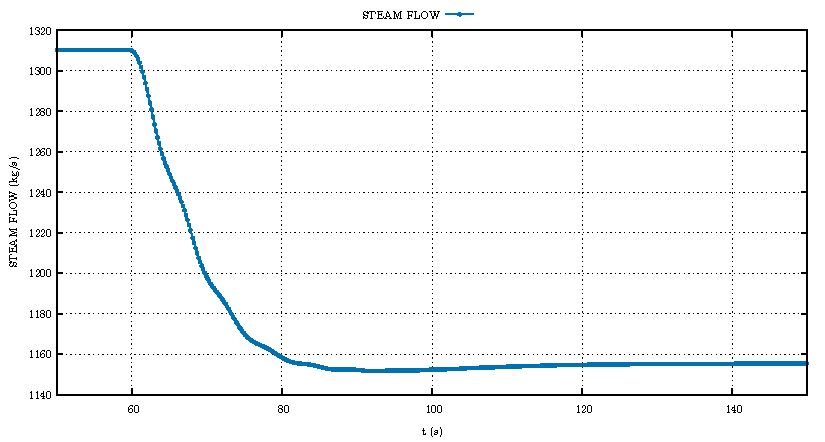
\includegraphics[width=\linewidth]{./graphs/STEAM FLOW_comp.pdf}
\end{figure}
\begin{figure}[H]
\centering
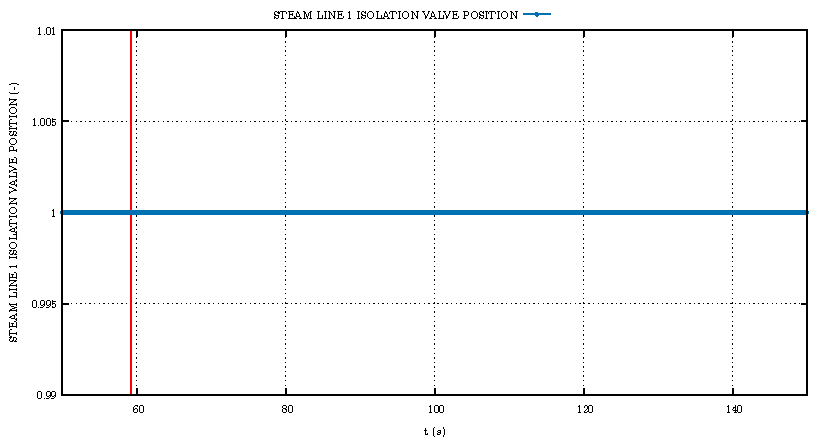
\includegraphics[width=\linewidth]{./graphs/STEAM LINE 1 ISOLATION VALVE POSITION_comp.pdf}
\end{figure}
\begin{figure}[H]
\centering
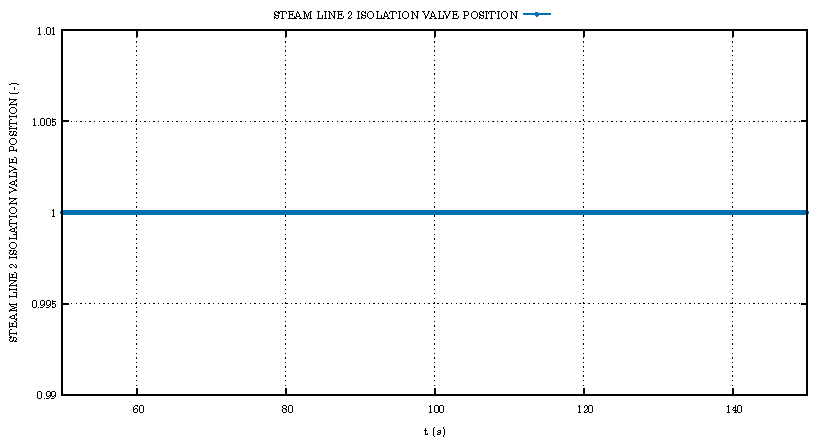
\includegraphics[width=\linewidth]{./graphs/STEAM LINE 2 ISOLATION VALVE POSITION_comp.pdf}
\end{figure}
\begin{figure}[H]
\centering
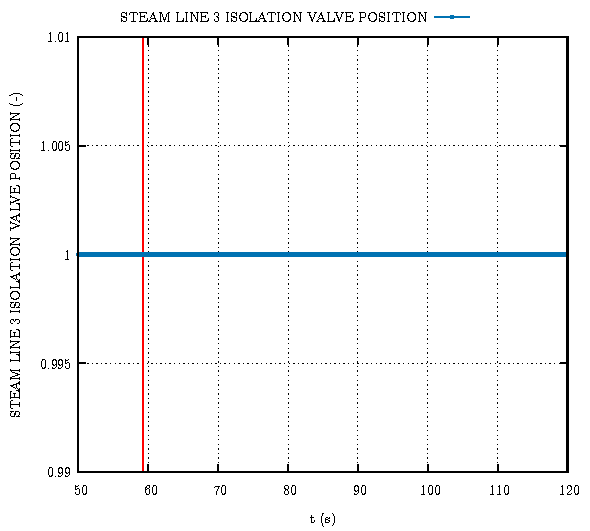
\includegraphics[width=\linewidth]{./graphs/STEAM LINE 3 ISOLATION VALVE POSITION_comp.pdf}
\end{figure}
\begin{figure}[H]
\centering
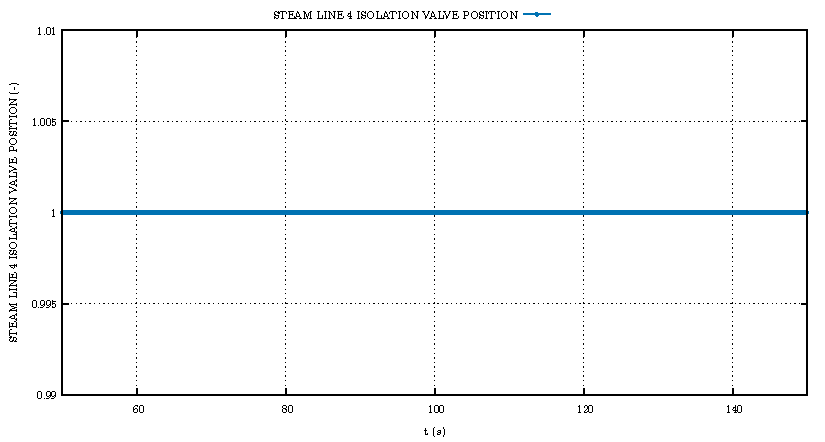
\includegraphics[width=\linewidth]{./graphs/STEAM LINE 4 ISOLATION VALVE POSITION_comp.pdf}
\end{figure}
\begin{figure}[H]
\centering
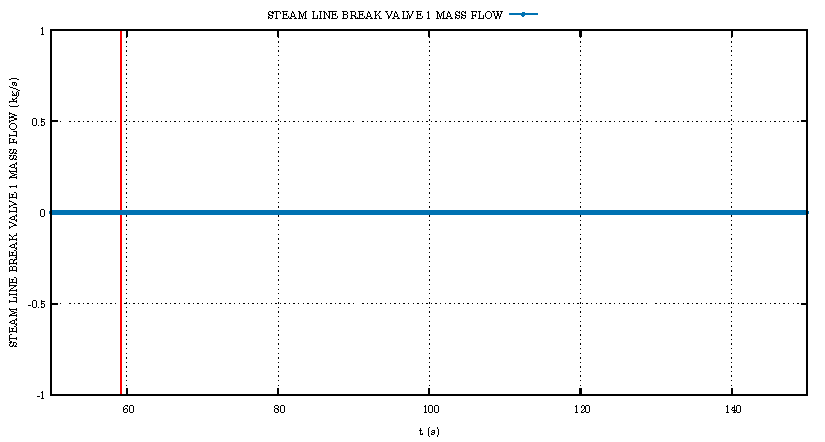
\includegraphics[width=\linewidth]{./graphs/STEAM LINE BREAK VALVE 1 MASS FLOW_comp.pdf}
\end{figure}
\begin{figure}[H]
\centering
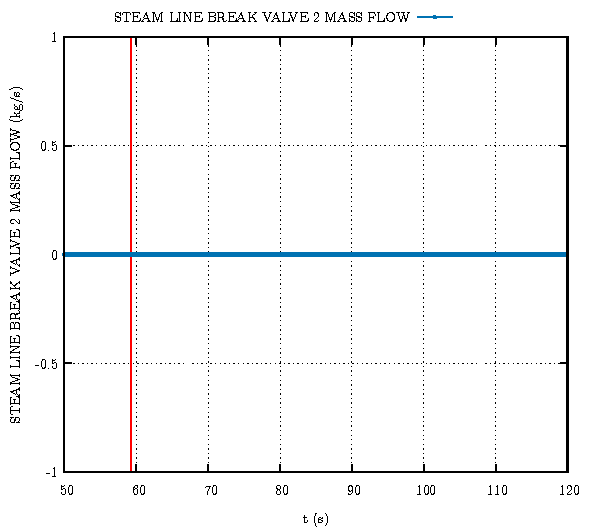
\includegraphics[width=\linewidth]{./graphs/STEAM LINE BREAK VALVE 2 MASS FLOW_comp.pdf}
\end{figure}
\end{multicols}
\end{document}
